\documentclass{article}

\usepackage{amsmath}
\usepackage{amsfonts}
\usepackage{amsthm}
\usepackage{nicefrac}
\usepackage{graphicx}
\usepackage{breqn}
\usepackage{tabularx}

\graphicspath{{./plots/}{./env/}{./results/}}
\usepackage[mode=buildnew]{standalone}


% DEFINITION/THEOREM ENVIRONMENTS
\newtheorem{theorem}{Theorem}
\newtheorem{problem}{Problem}
\newtheorem{olddefinition}{Definition}
\newtheorem{property}{Property}
\newtheoremstyle{named}{}{}{\itshape}{}{\bfseries}{:\\}{.5em}{#1 \thmnote{(#3)}}
\theoremstyle{named}
\newtheorem*{namedtheorem}{Theorem}
\newtheorem*{nameddefinition}{Definition}
\newtheorem*{namedproperty}{Property}

\newcommand{\thmsymbol}{\( \blacktriangle \)}
\newcommand{\propsymbol}{\( \blacklozenge \)}

\newenvironment{nameddef}[1]
    {\begin{samepage}
    \begin{nameddefinition}[#1]
    \renewcommand{\qedsymbol}{\thmsymbol}\pushQED{\qed}
    }
    {
    \popQED % in order to pop it before (in case of itemize) just call it in an item
    \end{nameddefinition} 
    \end{samepage}
    }
\newenvironment{namedprop}[1]
    {\begin{samepage}
    \begin{namedproperty}[#1]
    \renewcommand{\qedsymbol}{\propsymbol}\pushQED{\qed}
    }
    {
    \popQED % in order to pop it before (in case of itemize) just call it in an item
    \end{namedproperty} 
    \end{samepage}
    }
\newenvironment{namedtheo}[1]
    {\begin{samepage}
    \begin{namedtheorem}[#1]
    \renewcommand{\qedsymbol}{\propsymbol}\pushQED{\qed}
    }
    {
    \popQED % in order to pop it before (in case of itemize) just call it in an item
    \end{namedtheorem} 
    \end{samepage}
    }
\newenvironment{prop}[0]
    {\begin{samepage}
    \begin{property}
    \renewcommand{\qedsymbol}{\propsymbol}\pushQED{\qed}
    }
    {
    \popQED % in order to pop it before (in case of itemize) just call it in an item
    \end{property} 
    \end{samepage}
    }
\newenvironment{definition}[0]
    {\begin{samepage}
    \begin{olddefinition}
    \renewcommand{\qedsymbol}{\thmsymbol}\pushQED{\qed}
    }
    {
    \popQED % in order to pop it before (in case of itemize) just call it in an item
    \end{olddefinition} 
    \end{samepage}
    }
    
    
    
\usepackage[all]{xy}
\usepackage{amssymb}

\newdir{|>}{-{\scriptscriptstyle{\blacktriangleright}}}
\newcommand{\transition}{
  \ensuremath{ \xymatrix{\ar@{-|>}[r]&} }
  }
\newcommand{\labelledtransition}[1]{
  \ensuremath{ \xymatrix{\ar@{-|>}[r]^{#1}&} }
  }

\usepackage{nicefrac}
\newcommand{\vect}[1]{\ensuremath{ \mathbf{#1}}}
  


\usepackage{tikz}
\usetikzlibrary{shapes.geometric, arrows, positioning, calc, fit, arrows, decorations.pathreplacing}
\usepackage{pgfplots}
\usepackage{subcaption}


\usepackage{cite}

%\usepackage{showframe}
% use to create colored comments
\usepackage{xcolor}
\usepackage{color}
\usepackage{varwidth}
% guillemet are there because jstification wrong without them
\newcommand\comment[1]{\textcolor{red}{"\textit{#1}"}}

\begin{document}


\title{Experiment over the second integrator model}
\author{Paul Rousse}

\maketitle

\section{Notation}

For a matrix $A$ in $\mathbb{R}^{m \times n}$ let define respectively the image $Im(A) \subset \mathbb{R}^m$ and the kernel $ker(A) \subset \mathbb{R}^n$ by:
\begin{align*}
Im(A) &= \left \{ A \mathbf{x} \mid \mathbf{x}  \in \mathbb{R}^n \right \} \\ 
ker(A) &= \left \{ \mathbf{x} \in \mathbb{R}^n \mid A \mathbf{x} = 0\ \right \} 
\end{align*}

Let $dim(K)$ the dimension of the vectorial space $K$.
The Minkowski sum of $\mathcal{V},\mathcal{W} \subset X$ noted $\mathcal{V}+\mathcal{W}$ is the set $\left \{v+w \mid v \in \mathcal{V}, w\in \mathcal{W} \right \}$. We will use the abuse of notation $A  \mathcal{V} = \left \{ A \mathbf{x} \mid \mathbf{x}  \in \mathcal{V} \right \}$.

For $X$ a set, let $X^\star$ the set of finite or infinite sequence in $X$.

\section{Introduction}
As we will see in the experiments, when we model the quad as a single integrator, we hope that all the other behaviours 
The impact of the transient state is hidden in the noise modelling.
If we want to keep the abstraction controllable, we need to choose both a sampling time and a control that are large enough. However, this might not always be possible especially in small environments.
Therefore, we need to investigate a more complex model: the second integrator model with a feedback on the velocity.

The document aim also to compare the different abstraction methods.
How to evaluate the complexity of the model?
The answer of this question depend mainly of the use that we have of the abstraction. Fix points algorithms will have a complexity that is dependant mainly on the state space size (number of nodes).
In the case of path search algorithm (such as BFS or dijkstra), the search complexity depends also on the number of edges.

\section{Complexity of search algorithm}
What is the complexity of the search algorithm that I use?
We will use the BFS in order to compare the algorithms.

The complexity of the search algorithm will mainly lie in the branching factor.
The branching factor correspond to the average number of outgoing edges per node of the graph.
The complexity is then $\mathcal{O}(b^d)$ with $b$ the branching factor, $d$ the length of the path. 

For the following paragraphs, we will have a qualitative approach in order to know what are the impact of the different parameters on a complexity criteria.

\paragraph{Length of the path:}
Let $d_x$ the real distance that the dynamical model will do to reach the node.
Then the number of steps in the path (in the abstraction) will be $d = \nicefrac{d_x}{\left \| \Delta x_a \right \|}$ where  $\left \| \Delta x_a \right \|$ correspond to the average displacement of the system.

\paragraph{Nondeterministic behaviour:}
Lets define the nondeterministic branching factor $b_w$ the average branching of nondeterministic transition. $b_w = \frac{b}{b_u}$ where $b_u = \left | U \right |$ is the average number of inputs per states.

Lets define $V_d$ the volume of one cell of the state space discretization and $V_w$ the average volume due to the noise after $dt$. We have $b_w = \nicefrac{V_w}{V_d}$.

Therefore, we would like to build an abstraction that both respect the controllability property and minimize the criteria $b^d$ define as follow:
\begin{align*}
b   &= b_u b_w\\
b_w &= \frac{V_w}{V_d}\\
d &= \frac{d_x}{\left \| \Delta x_a \right \|}
\end{align*}

\paragraph{Final criteria}

So lets choose:
\begin{equation}
h = 	\frac{log(b_u V_w) -log(V_d) }{\left \| \Delta x_a \right \|}
\end{equation}
as a criteria for the abstraction.

\subsection{Noise branching factor}

We would like to see how much the number of successors increase when we choose one model.
\begin{align*}
\mathbf{x}_{n+1} &= A_d \mathbf{x}_n + B_d \mathbf{u}_n + E_d \mathbf{w}_n\\
V_{w} &= A_d V_d + B_d \mathbf{u}_n + E_d \mathcal{W}\\
\end{align*}

\section{Influence on the criteria}
We will consider a linear monotone systems:
\begin{equation}\label{eqn:lin_sys}
\begin{split}
\dot{\mathbf{x}} &= A \mathbf{x} + B \mathbf{u} + \mathbf{w}\\
\mathbf{y} &= \mathbf{x}
\end{split}
\end{equation}

Let the discrete model of system \ref{eqn:lin_sys} with a sampling time $\Delta t$:
\begin{equation}\label{eqn:disc_lin_sys}
\begin{split}
\mathbf{x}_{n+1} &= A_d \mathbf{x}_n + B_d \mathbf{u}_n+ E_d \mathbf{w}_n\\
\mathbf{y}_n &= \mathbf{x}_n
\end{split}
\end{equation}


In the following parts we will try to see what is the influence of the following transformation on the criteria:
\begin{itemize}
\item sampling time
\item reducing the number of states
\item increase the number of inputs over time (instead of using one inputs, choosing a past sequence of inputs).
\end{itemize}


\subsection{Sampling time}
\comment{TODO}

\section{Experiments}
We will use the system \ref{eqn:lin_sys} with the following parameters to model the quadricopter:
where
\begin{equation*} \label{eqn:sec_int}
A = \begin{bmatrix}
0 & 1\\ 
0 & -k
\end{bmatrix}
\textrm{, }
B = \begin{bmatrix}
0 \\ 
k 
\end{bmatrix}
\textrm{, }
C = \begin{bmatrix}
1 & 0\\ 
0 & 1
\end{bmatrix}
\textrm{, }
k \in \mathbb{R}_+^\star
\end{equation*}

We have been doing the synthesis of controller using different reduction of the second integrator model, we will compare the results to the raw second integrator model.
As we have seen in the previous parts, there is no need to test different values than the $\Delta n_u = 0$ and $\Delta n_u = 1$.
The case $\Delta n_u = 0$ (mode without any memories) correspond to the case of the single integrator.

After this presentation of the results, we will discuss when it is relevant to use each models.


\paragraph{Identification}
We would like to find the parameters of the system so that the system \ref{eqn:lin_sys} can be used as an abstraction for the model.
The velocity controller use the gain $k=2.0$.
The set $\mathcal{W}$ has been chosen so that for all the real trajectories of the system, we can find a $\mathbf{w} \in \mathcal{W}$ so that the equation \ref{eqn:disc_lin_sys} stand.

Please note that the observation noise is already modelled in the the state noise.

\comment{Things to explains:
\begin{itemize}
\item How to choose the sampling time
\item How to configure the model
\item Speed profiles (add the velocity commands)
\item Computation of the time
\end{itemize}
}

\subsection{First integrator model} \label{sec:single_int}

\begin{figure}[!ht]
	\begin{subfigure}[b]{0.5\textwidth}
  		\centering
  		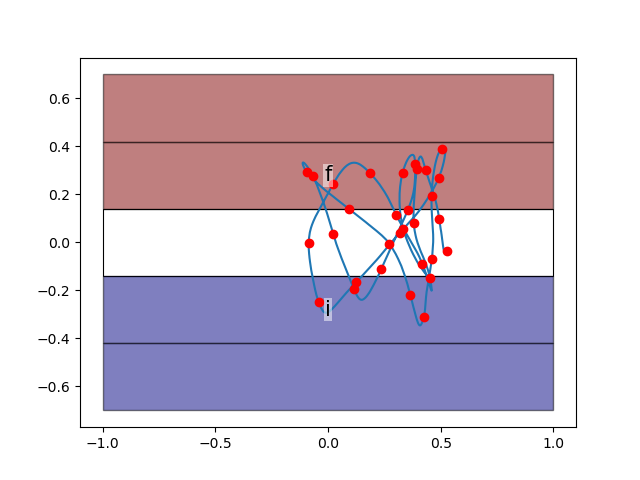
\includegraphics[width=0.9\linewidth]{simple_1D}
	  	\caption{Trajectory in the 2D environment.}
	  	\label{simple_1D}
  \end{subfigure}
	\begin{subfigure}[b]{0.5\textwidth}
  		\centering
  		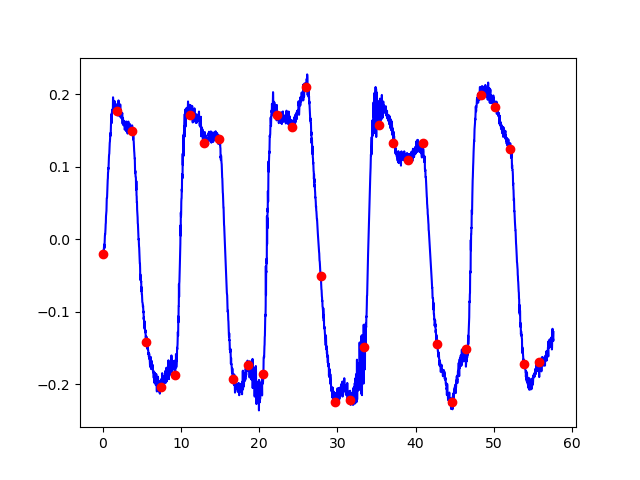
\includegraphics[width=0.9\linewidth]{simple_1D_vel}
	  	\caption{Velocity profile.}
	  	\label{simple_1D_vel}
  \end{subfigure}
  \caption{Trajectory and velocity profile of the simple integrator model with self loops. The agent is trying to achieve 'go infinity often to i and f'.}
\end{figure}

\begin{figure}[!ht]
	\begin{subfigure}[b]{0.5\textwidth}
  		\centering
  		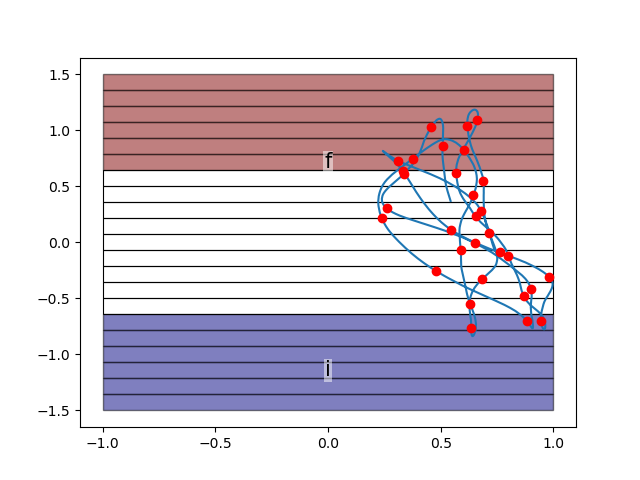
\includegraphics[width=0.9\linewidth]{simplenosl_1D}
	  	\caption{Trajectory in the 2D environment.}
	  	\label{simplenosl_1D}
  \end{subfigure}
	\begin{subfigure}[b]{0.5\textwidth}
  		\centering
  		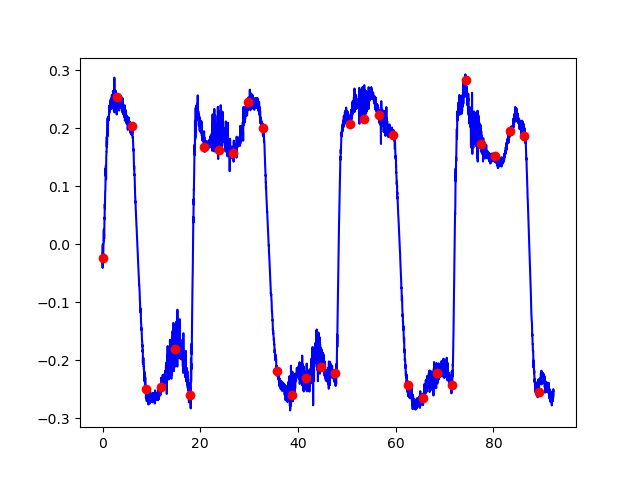
\includegraphics[width=0.9\linewidth]{simplenosl_1D_vel}
	  	\caption{Velocity profile.}
	  	\label{simplenosl_1D_vel}
  \end{subfigure}
  \caption{Trajectory and velocity profile of the simple integrator model without self loops. The agent is trying to achieve 'go infinity often to i and f'.}
\end{figure}

The first integrator model is the reduction of the second integrator model with velocity feedback in the case $\Delta n_u = 0$.
We have been choosing the sampling time so that the there is (figure \ref{simplenosl_1D}) no self-loops in the model or that there is self-loops (figure \ref{simple_1D}).

\newcommand{\reg}[1]{\textit{#1}}
Other constraints apply on the sampling time: regions \reg{i} and \reg{f} needs to be reachable. If the sampling time is too high, the state might miss the target region.

When using a sampling time close to the transient time of the system, the reduction needs to take in account more states that belong to the transient states. This result in an increase of the modelled noise in the first integrator model.

\subsection{Second integrator model with velocity feedback}

\begin{figure}[!ht]
	\begin{subfigure}[b]{0.5\textwidth}
  		\centering
  		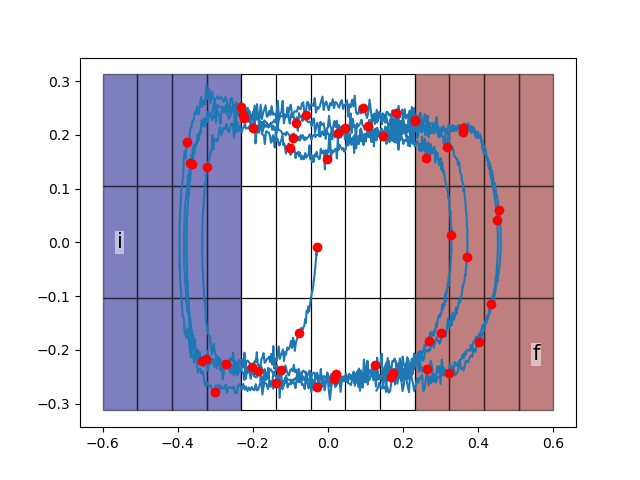
\includegraphics[width=0.9\linewidth]{double_1D}
	  	\caption{Trajectory in the 2D environment.}
	  	\label{double_1D}
  \end{subfigure}
	\begin{subfigure}[b]{0.5\textwidth}
  		\centering
  		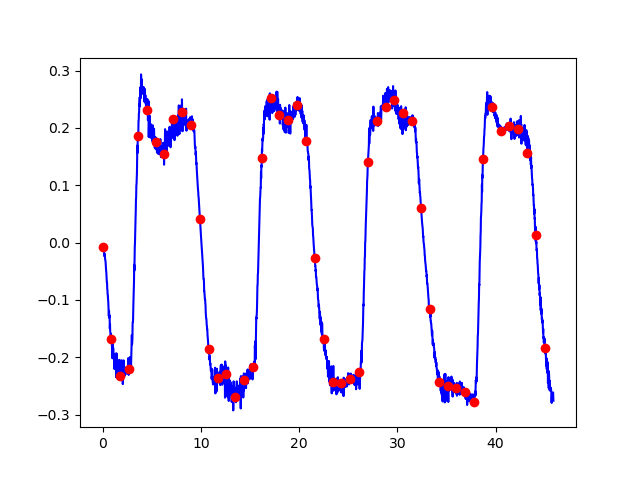
\includegraphics[width=0.9\linewidth]{double_1D_vel}
	  	\caption{Velocity profile.}
	  	\label{double_1D_vel}
  \end{subfigure}
  \caption{Trajectory and velocity profile of the double integrator model. The agent is trying to achieve 'go infinity often to i and f'.}
\end{figure}

We can see that the second integrator model manage to take in account the transient state that was hidden by the single integrator model: in $x\approx0.4$, the transient states is clearly going "backward", this show that this model is not usable with the single integrator model (which correspond to non reachability behaviours).

By matter of simplicity, the same upper bound has been used for the second integrator model.
The space discretization is chosen as follow:
the transient states cannot create self loops on the speed axis and on the position axis.
We need to discretize the state space enough so that there is not any self loops during the transient states. \comment{Why?}

\subsection{Second integrator model with velocity feedback reduced}

\begin{figure}[!ht]
	\begin{subfigure}[b]{0.5\textwidth}
  		\centering
  		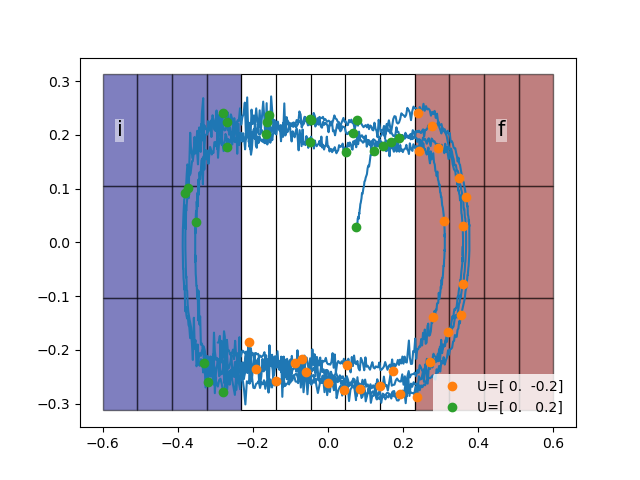
\includegraphics[width=\linewidth]{double_reduced_1D}
	  	\caption{Trajectory in the state space.}
	  	\label{double_reduced_1D}
  \end{subfigure}
	\begin{subfigure}[b]{0.5\textwidth}
  		\centering
  		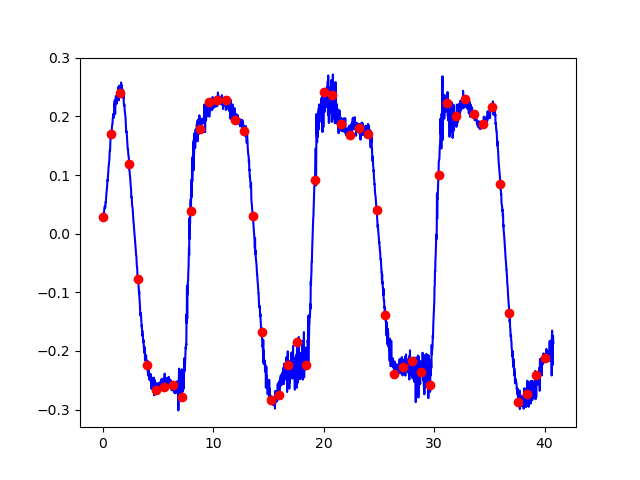
\includegraphics[width=\linewidth]{double_reduced_1D_vel}
	  	\caption{Velocity profile.}
	  	\label{double_reduced_1D_vel}
  \end{subfigure}
  \caption{Trajectory and velocity profile of the double integrator reduced model. The agent is trying to achieve 'go infinity often to i and f'.}
\end{figure}

Lets call $S$ the system \ref{eqn:lin_sys} with the following parameters:
\begin{equation*}\label{eqn:sec_int_reduced}
A = \begin{bmatrix}
0 & 1\\ 
0 & -k
\end{bmatrix}
\textrm{, }
B = \begin{bmatrix}
0 \\ 
k 
\end{bmatrix}
\textrm{, }
C = \begin{bmatrix}
1 & 0
\end{bmatrix}
\textrm{, }
k \in \mathbb{R}_+^\star
\end{equation*}

We have
\begin{align*}
ker(C_d) &=  \begin{bmatrix}
0\\ 
1
\end{bmatrix}\\
\dot{\mathbf{x}}_r &= A_r \mathbf{x}_r + B_r \mathbf{u}_r + E_r \mathbf{w}_r\\
\mathbf{x} &= \begin{bmatrix}
\mathbf{x}_z\\
\mathbf{x}_r
\end{bmatrix}\\
A_r &= \begin{bmatrix}
-k
\end{bmatrix}
\textrm{, }
B_r = \begin{bmatrix}
k
\end{bmatrix}
\textrm{, }
E_r = \begin{bmatrix}
1
\end{bmatrix}
\end{align*}


The reduced system is monotonic stable and the inputs of the reduced systems are bounded. Therefore it is possible to reduce the all system.

In our setup, the sampling time of model is ${\Delta t = 1s}$ and the timing constants of the reduced system is $\tau_r = {\nicefrac{1}{k} = 0.7s}$. This make relevant to use this reduction method as the internal dynamic of the quadricopter are not vanished enough after a $\Delta t$.


Comparison of the two results:
\begin{itemize}
\item compute the minimal number of states so that the model is usable (ie controllable)
\item compute the branching factor, the precision etc...
\item compute the amplitude of the noise in permanent state
\end{itemize}

Try to do it for different $\Delta n_u$, show that it does decrease the complexity for $\Delta n_u = 1$. Talk about the case $\Delta n_u = 0$ which correspond to the single integrator case (see part \ref{sec:single_int}).

Comparison to the double integrator case, show how the noise is evolving. Compare the size of the successors between the case where the discretization of the reduced state (velocity in this case) is lower than the steady state of the reduced state for a stable sequence. Basically, in one case, the size of the successors is growing (expansion of the successors) in the reduced approach, the size of the successors is reducing (but is bigger than the other one).


\comment{Try to show the 2 abstractions on top of each other to visualize what happened after the reduction}.

\paragraph{Sensitivity to noise}:
Please note that this model is less sensible to the noise on velocity as only the position is observed.
We have been noticing that this model was much easier to use thanks to this property.

\subsection{Experiments over 2 axes}

The previous study show the link between the precision and the complexity of the abstraction that we used.
In this part we will use the previous results in order to solve the following problem for different size of the environment:

\begin{figure}
	\center
	\includestandalone[width=0.5\textwidth]{2D_env_problem}
	\caption{Testing environment for the quadricopter.}
	\label{fig:environment}
\end{figure}

\comment{Show the simulation, the runs and so on.}


\subsection{Real case scenarios}

\begin{figure}[!ht]
  \centering
  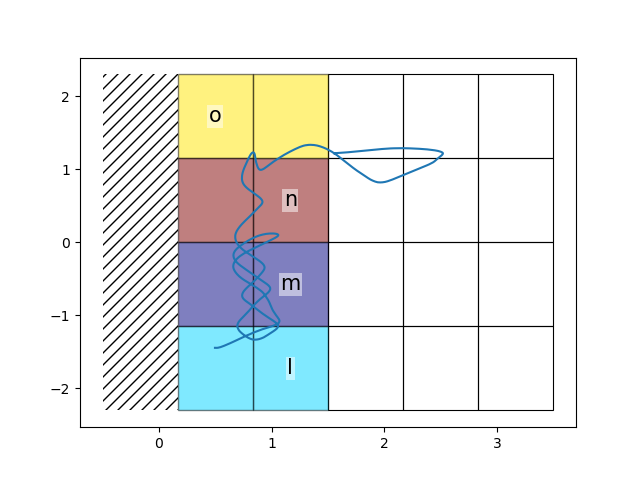
\includegraphics[width=0.9\linewidth]{real_case_scenarios}
  \caption{A trajectory in the state space $(x,v)$.}
\end{figure}

We have been using the first integrator model in this case (this is the more relevant in the scenario of the wind power).

\subsection{Discussion over the different models}
See table \ref{comparaison_table}.

\paragraph{Method:}
the comparison the different abstractions does not make any sense.
For example, in the second integrator abstraction, the discretization of the state space can be chosen to be the same than the reduced model, but we can always increase the precision over the velocity state.
We need to find a method that does not depend on a wrong parametrization of the method. Maybe defined the way we have been choosing the different abstraction (optimization criteria)?
So we need to use a standardized method in order to compare them.
For example, the minimum controllable abstraction might be a good choice.

There is no better abstraction, so we need to play with the parameters to show in which case the reduction is better than the original model.


\paragraph{Comparison for the second integrator model over 1 dimension:} in this paragraph, we are going to investiguate when each model are better than each other.
We will compare 3 different models:
the second integrator model,
the reduced model of the second integrator ($\Delta n_u = 1$)
and the single integrator model (which is equivalent to the second integrator reduced model with $\Delta n_u = 0$).
In each cases, we will choose the optimal discretization. These tests are made in 1 dimension in order to be able to work with the 3 models (the complexity might be sometime too high for them).

These study is supposed to give us a good inside in what to do.

I have been working on different models mainly because the size of the environment is  too small for using a single integrator.


Figures \ref{fig:compare_cpu} and \ref{fig:compare_dt} show the comparison between the different models. We have been running algorithm to search for the smallest (in term of nodes) abstraction for different models: the second integrator with velocity feedback, the reduced model with $\Delta n_u = 1$ and $\Delta n_u = 0$.
As we have seen in the previous sections, the reduction can hide the transient state of the intial model and reduce the size of the abstraction.
These results are showing this.
When the size of the environment is too small, the transient state of the single integrator is making the all model uncontrollable and w are not able to find any solution to the problem.
By adding some states to take in account the transient state, we can find a solution to the problem for $L<|u| \lambda$. Both the second integrator model and the 1-input reduced model are usable in this situation, however, the discretization of the velocity in the second integrator model most of the time is the "same" than the reduced model. So I believe that the reduced model is finding directly the optimal abstraction in this case.
On the 2 figures, the vertical lines correspond to limits where we were not able to find valid abstraction in these area. In the case of the single integrator without loops, it correspond to the limits where any decrease of the sampling time create self-loops,. For the single integrator with self-loops, it correspond to controllability issues. For 2 other models, it might be more complex to understand.

\comment{I need to add the single integrator without self-loops in order to show when it is better to use it instead of the single integrator.}
\comment{talk about typical distances that make sense to compare the abstraction to.}
\comment{Try to determine what is extrem size where we will not be able to control the plant (by taking an infinite precise abstraction). To show until when it is smart to perform the study.}


\pgfplotstableread{
a N_pos CPU_time diam nc b_pos L edges v_max nodes N_vel sl found max_fixed_point_size deg dt b_vel
1.00e-01 22 1.69e+01 13 9.02e+00 1.00e-02 0.063095734448019331 3620 1.05e-01 244 13 5.16e-01 1 2 4.95e+00 0.17692307692307691 1.00e-02
1.00e-01 18 5.46e+00 14 7.98e+00 1.00e-02 0.085769589859089418 1874 1.05e-01 168 11 6.07e-01 1 2 3.72e+00 0.19090909090909092 1.00e-02
1.00e-01 6 7.07e-02 5 2.10e+00 1.00e-02 0.11659144011798317 158 1.05e-01 20 5 1.00e+00 1 2 2.63e+00 0.40000000000000002 1.00e-02
1.00e-01 6 2.98e-02 5 1.19e+00 1.00e-02 0.15848931924611137 52 1.05e-01 10 3 1.00e+00 1 2 1.73e+00 0.53333333333333344 1.00e-02
1.00e-01 6 2.59e-02 5 1.19e+00 1.00e-02 0.21544346900318839 52 1.05e-01 10 3 1.00e+00 1 2 1.73e+00 0.53333333333333344 1.00e-02
1.00e-01 4 1.92e-02 3 5.76e-01 1.00e-02 0.29286445646252368 28 1.05e-01 6 3 1.00e+00 1 2 1.56e+00 1.1333333333333335 1.00e-02
1.00e-01 4 1.89e-02 3 5.76e-01 1.00e-02 0.39810717055349731 28 1.05e-01 6 3 1.00e+00 1 2 1.56e+00 1.1333333333333335 1.00e-02
1.00e-01 4 1.95e-02 3 5.76e-01 1.00e-02 0.54116952654646377 28 1.05e-01 6 3 1.00e+00 1 2 1.56e+00 1.0333333333333334 1.00e-02
1.00e-01 4 2.01e-02 3 5.76e-01 1.00e-02 0.73564225445964138 28 1.05e-01 6 3 1.00e+00 1 2 1.56e+00 1.1333333333333335 1.00e-02
1.00e-01 4 1.88e-02 3 5.76e-01 1.00e-02 1.0 28 1.05e-01 6 3 1.00e+00 1 2 1.56e+00 1.1333333333333335 1.00e-02
} \datadouble

\pgfplotstableread{
a                     CPU_time  b                     nc         nodes  L                     edges  N  diam  sl        dt                   max_fixed_point_size  deg
0.061562757024726023 1.07e-02 0.053437242975273962 -3.27e-01 3 0.20309176209047358 7 4 3 1.00e+00 1.1773435408566417 2 7.78e-01
0.066564806686465611 9.60e-03 0.048435193313534394 -3.27e-01 3 0.24244620170823283 7 4 3 1.00e+00 1.4054852272941025 2 7.78e-01
0.071239311624347129 1.53e-02 0.043760688375652876 -3.27e-01 3 0.28942661247167517 7 4 3 1.00e+00 1.6778354346184061 2 7.78e-01
0.07549146940430515 1.34e-02 0.039508530595694882 -3.27e-01 3 0.34551072945922201 7 4 3 1.00e+00 2.0029607504882421 2 7.78e-01
0.079264202173056367 1.04e-02 0.035735797826943631 -3.27e-01 3 0.41246263829013524 7 4 3 1.00e+00 2.3910877582036765 2 7.78e-01
0.082541429295829152 1.26e-02 0.03245857070417088 -3.27e-01 3 0.49238826317067413 7 4 3 1.00e+00 2.854424714032886 2 7.78e-01
0.085342779834559082 inf 0.02965722016544093 0.00e+00 3 0.58780160722749153 9 4 2 1.00e+00 3.4075455491448792 2 1.00e+00
0.087712089589932069 1.38e-02 0.02728791041006794 -3.27e-01 3 0.70170382867038295 7 4 3 1.00e+00 4.0678482821471471 2 7.78e-01
0.089704299805719326 inf 0.0252957001942807 0.00e+00 3 0.83767764006829204 9 4 2 1.00e+00 4.8561022612654607 2 1.00e+00
0.091375079517141883 1.11e-02 0.023624920482858119 -3.27e-01 3 1.0 7 4 3 1.00e+00 5.7971014492752149 2 7.78e-01
0.092775037398332053 1.36e-02 0.022224962601667984 -3.27e-01 3 1.1937766417144369 7 4 3 1.00e+00 6.9204442997937541 2 7.78e-01
0.093947804881452393 8.95e-03 0.021052195118547615 -3.27e-01 3 1.4251026703029992 7 4 3 1.00e+00 8.2614647553796381 2 7.78e-01
0.094930211151424457 inf 0.020069788848575569 0.00e+00 3 1.7012542798525891 9 4 2 1.00e+00 9.8623436513193568 2 1.00e+00
0.095753151230405009 8.73e-03 0.01924684876959501 -3.27e-01 3 2.030917620904737 7 4 3 1.00e+00 11.773435483505242 2 7.78e-01
0.096442509744749647 1.59e-02 0.018557490255250341 -3.27e-01 3 2.4244620170823281 7 4 3 1.00e+00 14.054852272940501 2 7.78e-01
0.097019969958414221 8.19e-03 0.017980030041585791 -3.27e-01 3 2.8942661247167516 7 4 3 1.00e+00 16.778354346184024 2 7.78e-01
0.097503695467431803 1.04e-02 0.017496304532568202 -3.27e-01 3 3.4551072945922217 7 4 3 1.00e+00 20.029607504882438 2 7.78e-01
0.097908901510266516 1.37e-02 0.017091098489733517 -3.27e-01 3 4.1246263829013525 7 4 3 1.00e+00 23.910877582036818 2 7.78e-01
0.098248333551969616 1.50e-02 0.016751666448030406 -3.27e-01 3 4.9238826317067419 7 4 3 1.00e+00 28.544247140327858 2 7.78e-01
0.09853266818362616 1.40e-02 0.016467331816373859 -3.27e-01 3 5.878016072274912 7 4 3 1.00e+00 34.075455491425771 2 7.78e-01
0.098770848946862846 1.55e-02 0.016229151053137145 -3.27e-01 3 7.0170382867038299 7 4 3 1.00e+00 40.678482821444796 2 7.78e-01
0.098970367646518495 1.54e-02 0.016029632353481541 -3.27e-01 3 8.3767764006829246 7 4 3 1.00e+00 48.561022612520958 2 7.78e-01
0.099137499999999282 1.18e-02 0.015862500000000695 -3.27e-01 3 10.0 7 4 3 1.00e+00 57.971014492706857 2 7.78e-01
} \datasimple

\pgfplotstableread{
a N_pos CPU_time diam nc b_pos L v_max nodes edges sl found max_fixed_point_size deg dt b_vel
1.00e-01 6 3.34e-02 5 1.92e+00 1.00e-02 0.083767764006829198 1.05e-01 15 109 1.00e+00 1 1 2.42e+00 0.28999999999999992 1.00e-02
1.00e-01 6 3.27e-02 5 1.92e+00 1.00e-02 0.10000000000000001 1.05e-01 15 109 1.00e+00 1 1 2.42e+00 0.28999999999999992 1.00e-02
1.00e-01 6 3.29e-02 5 1.92e+00 1.00e-02 0.1193776641714437 1.05e-01 15 109 1.00e+00 1 1 2.42e+00 0.29999999999999993 1.00e-02
1.00e-01 6 3.39e-02 5 1.92e+00 1.00e-02 0.14251026703029984 1.05e-01 15 109 1.00e+00 1 1 2.42e+00 0.28999999999999992 1.00e-02
1.00e-01 6 3.26e-02 5 1.92e+00 1.00e-02 0.17012542798525893 1.05e-01 15 109 1.00e+00 1 1 2.42e+00 0.28999999999999992 1.00e-02
1.00e-01 6 3.17e-02 5 1.92e+00 1.00e-02 0.20309176209047358 1.05e-01 15 109 1.00e+00 1 1 2.42e+00 0.28999999999999992 1.00e-02
1.00e-01 3 1.74e-02 3 5.76e-01 1.00e-02 0.24244620170823283 1.05e-01 6 28 1.00e+00 1 1 1.56e+00 1.0299999999999996 1.00e-02
1.00e-01 3 2.00e-02 3 5.76e-01 1.00e-02 0.28942661247167517 1.05e-01 6 28 1.00e+00 1 1 1.56e+00 1.0299999999999996 1.00e-02
1.00e-01 3 2.28e-02 3 5.76e-01 1.00e-02 0.34551072945922201 1.05e-01 6 28 1.00e+00 1 1 1.56e+00 1.0399999999999996 1.00e-02
1.00e-01 3 1.90e-02 3 5.76e-01 1.00e-02 0.41246263829013524 1.05e-01 6 28 1.00e+00 1 1 1.56e+00 1.0399999999999996 1.00e-02
1.00e-01 3 1.89e-02 3 5.76e-01 1.00e-02 0.49238826317067413 1.05e-01 6 28 1.00e+00 1 1 1.56e+00 1.0399999999999996 1.00e-02
1.00e-01 3 2.24e-02 3 5.76e-01 1.00e-02 0.58780160722749153 1.05e-01 6 28 1.00e+00 1 1 1.56e+00 1.0499999999999996 1.00e-02
1.00e-01 3 2.11e-02 3 5.76e-01 1.00e-02 0.70170382867038295 1.05e-01 6 28 1.00e+00 1 1 1.56e+00 1.0299999999999996 1.00e-02
1.00e-01 3 2.21e-02 3 5.76e-01 1.00e-02 0.83767764006829204 1.05e-01 6 28 1.00e+00 1 1 1.56e+00 1.0299999999999996 1.00e-02
1.00e-01 3 1.87e-02 3 5.76e-01 1.00e-02 1.0 1.05e-01 6 28 1.00e+00 1 1 1.56e+00 1.0299999999999996 1.00e-02
1.00e-01 3 2.29e-02 3 5.76e-01 1.00e-02 1.1937766417144369 1.05e-01 6 28 1.00e+00 1 1 1.56e+00 1.0299999999999996 1.00e-02
1.00e-01 3 1.95e-02 3 5.76e-01 1.00e-02 1.4251026703029992 1.05e-01 6 28 1.00e+00 1 1 1.56e+00 1.0399999999999996 1.00e-02
1.00e-01 3 1.88e-02 3 5.76e-01 1.00e-02 1.7012542798525891 1.05e-01 6 28 1.00e+00 1 1 1.56e+00 1.0299999999999996 1.00e-02
1.00e-01 3 2.01e-02 3 5.76e-01 1.00e-02 2.030917620904737 1.05e-01 6 28 1.00e+00 1 1 1.56e+00 1.0299999999999996 1.00e-02
1.00e-01 3 1.85e-02 3 5.76e-01 1.00e-02 2.4244620170823281 1.05e-01 6 28 1.00e+00 1 1 1.56e+00 1.0299999999999996 1.00e-02
1.00e-01 3 1.77e-02 3 5.76e-01 1.00e-02 2.8942661247167516 1.05e-01 6 28 1.00e+00 1 1 1.56e+00 1.0299999999999996 1.00e-02
1.00e-01 3 1.68e-02 3 5.76e-01 1.00e-02 3.4551072945922217 1.05e-01 6 28 1.00e+00 1 1 1.56e+00 1.0599999999999996 1.00e-02
1.00e-01 3 1.98e-02 3 5.76e-01 1.00e-02 4.1246263829013525 1.05e-01 6 28 1.00e+00 1 1 1.56e+00 1.0399999999999996 1.00e-02
1.00e-01 3 1.89e-02 3 5.76e-01 1.00e-02 4.9238826317067419 1.05e-01 6 28 1.00e+00 1 1 1.56e+00 1.0299999999999996 1.00e-02
1.00e-01 3 1.68e-02 3 5.76e-01 1.00e-02 5.878016072274912 1.05e-01 6 28 1.00e+00 1 1 1.56e+00 1.0299999999999996 1.00e-02
1.00e-01 3 1.72e-02 3 5.76e-01 1.00e-02 7.0170382867038299 1.05e-01 6 28 1.00e+00 1 1 1.56e+00 1.0299999999999996 1.00e-02
1.00e-01 3 1.92e-02 3 5.76e-01 1.00e-02 8.3767764006829246 1.05e-01 6 28 1.00e+00 1 1 1.56e+00 1.0299999999999996 1.00e-02
1.00e-01 3 1.88e-02 3 5.76e-01 1.00e-02 10.0 1.05e-01 6 28 1.00e+00 1 1 1.56e+00 1.0299999999999996 1.00e-02
}\datadoublereduced

\pgfplotstableread{
a CPU_time b nc nodes L edges N diam sl dt max_fixed_point_size deg
0.086743962080486847 2.05e-02 0.02825603791951314 7.04e-01 6 0.6614740641230149 18 7 4 0.00e+00 3.7698611790641157 1 1.50e+00
0.088794088924601861 2.37e-02 0.026205911075398158 7.04e-01 6 0.83767764006829182 18 7 4 0.00e+00 4.4613359045078536 1 1.50e+00
0.090630820535082673 2.53e-02 0.024369179464917332 7.04e-01 6 1.0608183551394483 18 7 4 0.00e+00 5.3365230267374288 1 1.50e+00
0.092241709569416269 2.24e-02 0.022758290430583712 7.04e-01 6 1.3433993325989002 18 7 4 0.00e+00 6.4447025043048729 1 1.50e+00
0.092962706555600738 2.18e-02 0.022037293444399246 7.04e-01 6 1.5117750706156623 18 7 4 0.00e+00 7.1049994850725771 1 1.50e+00
0.093628996364086919 1.98e-02 0.021371003635913103 7.04e-01 6 1.7012542798525891 18 7 4 0.00e+00 7.8480558531205054 1 1.50e+00
0.094242445954468165 2.59e-02 0.020757554045531833 7.04e-01 6 1.9144819761699576 18 7 4 0.00e+00 8.6842430262270494 1 1.50e+00
0.094805321161505987 2.23e-02 0.020194678838494035 7.04e-01 6 2.1544346900318834 18 7 4 0.00e+00 9.6252340782677397 1 1.50e+00
0.09532017700657186 2.53e-02 0.019679822993428134 7.04e-01 6 2.4244620170823281 18 7 4 0.00e+00 10.684164773749639 1 1.50e+00
0.095789763406779194 2.43e-02 0.019210236593220808 7.04e-01 6 2.7283333764867681 18 7 4 0.00e+00 11.875817163835599 1 1.50e+00
0.096216943462902216 1.76e-02 0.018783056537097793 7.04e-01 6 3.0702906297578498 18 7 4 0.00e+00 13.216826000224767 1 1.50e+00
0.096604624315970736 1.94e-02 0.018395375684029276 7.04e-01 6 3.4551072945922181 18 7 4 0.00e+00 14.725910960361578 1 1.50e+00
0.096955700194912842 2.48e-02 0.018044299805087146 7.04e-01 6 3.8881551803080874 18 7 4 0.00e+00 16.424137963168967 1 1.50e+00
0.097273006899109782 2.33e-02 0.01772699310089023 7.04e-01 6 4.3754793750741845 18 7 4 0.00e+00 18.335213236761511 1 1.50e+00
0.097559286665079209 2.04e-02 0.017440713334920803 7.04e-01 6 4.9238826317067392 18 7 4 0.00e+00 20.485814243163674 1 1.50e+00
0.097817162194447568 2.06e-02 0.017182837805552461 7.04e-01 6 5.5410203300094922 18 7 4 0.00e+00 22.905962079645072 1 1.50e+00
0.098049118555969789 2.58e-02 0.016950881444030255 7.04e-01 6 6.2355073412739124 18 7 4 0.00e+00 25.62944055519182 1 1.50e+00
0.098257491692691309 1.89e-02 0.016742508307308706 7.04e-01 6 7.0170382867038263 18 7 4 0.00e+00 28.694267792171864 1 1.50e+00
0.098444462340423255 2.07e-02 0.016555537659576753 7.04e-01 6 7.8965228684997246 18 7 4 0.00e+00 32.143226936469503 1 1.50e+00
0.098612054273609681 2.62e-02 0.016387945726390338 7.04e-01 6 8.8862381627434033 18 7 4 0.00e+00 36.02446338448393 1 1.50e+00
0.098762135922366129 2.27e-02 0.016237864077633859 7.04e-01 6 10.0 18 7 4 0.00e+00 40.392156863921578 1 1.50e+00
}\datasimplenosl



\begin{figure}
\center
\begin{tikzpicture}[scale=1]
\begin{axis}[
minor tick num=0,
ylabel near ticks,
xlabel=Size of the environment (m),
ylabel=CPU Time ($s$),
xmode=log,
ymode=log,
legend pos=north east,
legend cell align=left,
mark size=1.5,
legend style = {row sep=-4pt}]
\addplot [black,mark=x] table [x={L}, y={CPU_time}] {\datasimple};
\addplot [black,mark=+] table [x={L}, y={CPU_time}] {\datasimplenosl};
\addplot [black,mark=*] table [x={L}, y={CPU_time}] {\datadouble};
\addplot [black,mark=o] table [x={L}, y={CPU_time}] {\datadoublereduced};

\draw [very thin,dashed] ({axis cs:0.0837,0}|-{rel axis cs:0,1}) -- ({axis cs:0.0837,0}|-{rel axis cs:0,0});
\draw [very thin,dashed] ({axis cs:0.203,0}|-{rel axis cs:0,1}) -- ({axis cs:0.203,0}|-{rel axis cs:0,0});
\draw [very thin,dashed] ({axis cs:0.66,0}|-{rel axis cs:0,1}) -- ({axis cs:0.66,0}|-{rel axis cs:0,0});

\draw [<-]({axis cs:0.05,2}) -- ({axis cs:0.0837,2}) node[anchor=west] {double int};
\draw [<->]({axis cs:0.0837,1}) -- ({axis cs:0.203,1}) node[anchor=west] {1-input reduced};
\draw [->]({axis cs:0.203,0.5}) -- ({axis cs:0.403,0.5}) node[anchor=west] {0-input reduced} ;
\draw [->]({axis cs:0.66,0.25}) -- ({axis cs:1.2,0.25}) node[anchor=mid west,align=left,text width=3.cm] {0-input reduced without self-loops} ;

\legend{$1^{st}$ int,$1^{st}$ int no sl,$2^{sd}$ int,$2^{sd}$ int reduced}
\end{axis}
\end{tikzpicture}
\caption{Computation time of each models for different sizes of the environment}
\label{fig:compare_cpu}
\end{figure}

\begin{figure}
\center
\begin{tikzpicture}[scale=1]
\begin{axis}[
minor tick num=0,
ylabel near ticks,
xlabel=Size of the environment (m),
ylabel=Sampling time ($s$),
xmode=log,
ymode=log,
legend pos=north west,
legend cell align=left,
mark size=1,
legend style = {row sep=-4pt}]
\addplot [black,mark=*] table [x={L}, y={dt}] {\datasimple};
\addplot [black,mark=o] table [x={L}, y={dt}] {\datasimplenosl};
\addplot [black,mark=x] table [x={L}, y={dt}] {\datadouble};
\addplot [black,mark=+] table [x={L}, y={dt}] {\datadoublereduced};
\legend{$1^{st}$ int,$1^{st}$ int no sl,$2^{sd}$ int,$2^{sd}$ int reduced}
\end{axis}
\end{tikzpicture}
\caption{Complexity of the different abstractions for different size of the environment. Here the single integrator can be build as a double integrator reduced model with $\Delta n_u=0$.}
\label{fig:compare_dt}
\end{figure}


\bibliography{bibliography}{}
\bibliographystyle{plain}


\end{document}